% !TeX TXS-program:compile = txs:///pdflatex/[--shell-escape]

\documentclass[9pt]{beamer}
\usetheme{Madrid}
\usecolortheme{beaver}
\usepackage{amsmath,amssymb,amsthm,asymptote,graphicx}
\usepackage{graphics}
% \usepackage{bisvslides}
\usepackage{arcs}
\graphicspath{{./images}}

\newcounter{problem}[section]

% \newenvironment{probslide}[3][]{%
%     \refstepcounter{problem}\begin{frame}[t]%
% 	{Problem \thesection.\theproblem 
%         \def\temp{#2}\ifx\temp\empty
%             %
%         \else
%             \ - \temp%
%         \fi}
%     {#3}}%
% 	{\end{frame}}

% \newenvironment{Example}[2][Example]
%     {This is an #1. You gave #2 as an argument. The rest will be bold: \bfseries}
%     {}
% \textbf{Problem~\theproblem. #1
% \newenvironment{bsmi}{\begin{CJK}{UTF8}{bsmi}}{\end{CJK}}

\title{Counting and Probability}
\subtitle{Mathcounts 21 - Session 4}
\author{Derrick L., Maggie S.}
\institute{BISV Mathcounts Club 21}
\date{December 14, 2021}

%\maketitle
%~~~~~~~~~~~~~~~~~~~~~~~~~~~~~~~~~~~~~~~~~~~~~~~~~~~~~~~~~~~~~~~~~~~~~~~~~~~~~~
% Informations
%\title{TEMPLATE}

%\titlegraphic{assets/gkg.png} %change this to your preferred logo or image(the image is located on the top right corner).
%~~~~~~~~~~~~~~~~~~~~~~~~~~~~~~~~~~~~~~~~~~~~~~~~~~~~~~~~~~~~~~~~~~~~~~~~~~~~~~

\begin{document}

% Generate title page
\begin{frame}
    \titlepage        
\end{frame}
% \setbeamertemplate{footline}[miniframes Madrid]

\setcounter{section}{4}

\section{Beginner Practice Problems}
\refstepcounter{problem}
\begin{frame}[t, fragile]{Problem \thesection.\theproblem}
    \begin{block}{}[Mathcounts]
% Concept: Counting and Probability • Difficulty: 3 • Answer: 90 3-digit numbers • Solution Available: No • Report an error with this problem.
 Numbers that read the same forward or backward are called palindromes. How many three-digit numbers are palindromes?
	
    \end{block}
\end{frame}

\refstepcounter{problem}
\begin{frame}[t, fragile]{Problem \thesection.\theproblem}
    \begin{block}{}[Mathcounts]
    % Concept: Counting and Probability • Difficulty: 3 • Answer: 4200 • Solution Available: No • Report an error with this problem.
    How many arrangements of all eight letters in $TRESPASS$ do not have $S$ as the final letter?
	
    \end{block}
\end{frame}

\refstepcounter{problem}
\begin{frame}[t, fragile]{Problem \thesection.\theproblem}
    \begin{block}{}[Mathcounts]
    % Concept: Counting and Probability • Difficulty: 3 • Answer: 11/204 • Solution Available: Yes (Hide) • Report an error with this problem. 
    Jorge has a bag with $6$ red marbles and $12$ blue marbles. He randomly selects $4$ marbles from the bag, one at a time without replacement. What is the probability that he selects $2$ red marbles followed by $2$ blue marbles? Express your answer as a common fraction.

	
    \end{block}
\end{frame}

\refstepcounter{problem}
\begin{frame}[t, fragile]{Problem \thesection.\theproblem}
    \begin{block}{}[Mathcounts]
% Concept: Counting and Probability • Difficulty: 3 • Answer: 8/9 • Solution Available: Yes (Hide) • Report an error with this problem.
 Bob and Meena play a two-person game which is won by the first person to accumulate 10 points. At each turn Bob gains a point with probability of $\frac{1}{3}$ . If he doesn't get a point, then Meena gets a point. Meena is now ahead 9 to 8. What is the probability that Meena will win? Express your answer as a common fraction.
    \end{block}
\end{frame}
 
\refstepcounter{problem}
\begin{frame}[t, fragile]{Problem \thesection.\theproblem}
    \begin{block}{} [Mathcounts Handbook 2021-2022, \#240]
% Concept: Counting and Probability • Difficulty: 3 • Answer: 1/15 • Solution Available: Yes (Hide) • Report an error with this problem.
 Three pairs of sisters stand in a line in a random order. What is the probability that everybody in the line is adjacent to her sister? Express your answer as a common fraction.	
    \end{block}
\end{frame}

\refstepcounter{problem}
\begin{frame}[t, fragile]{Problem \thesection.\theproblem}
    \begin{block}{}[Mathcounts]
% Concept: Counting and Probability • Difficulty: 3 • Answer: 3/8 • Solution Available: No • Report an error with this problem.
 Boris starts at point $B$---the farthest point north---and walks toward the bottom, randomly heading southeast or southwest, until he reaches one of the five points. What is the probability he will arrive at point $R$? Express your answer as a common fraction.
    \end{block}
    \begin{center}
        \begin{asy}
            size(150); 
            pair left = dir(-135); pair right = dir(-45); fontsize(10pt);
            pair B = (0,0), P = 4left, Q = 3left + right, R = 2left + 2right, S = left + 3right, T = 4right;
            
            draw(B--P ^^ 3left--Q--right ^^ 2left--R--2right ^^ left--S--3right ^^ B--T);
            label("$B$",B,N); void labeler(string s,pair loc) {label("$"+s+"$",loc,(0,-1));} labeler("P",P); labeler("Q",Q); labeler("R",R); labeler("S",S); labeler("T",T);
            
            picture compass; real length = .5, lengthshort = .1,frac = .2,scaleforpoints = 4;
            pair east = length*(1,0), north = length*(0,1), west = length*(-1,0), south = length*(0,-1);
            pair northeast = lengthshort*NE, northwest = lengthshort*NW, southwest = lengthshort*SW, southeast = lengthshort*SE;
            draw(compass, east--northeast--north--northwest--west--southwest--south--southeast--cycle);
            pair weighted(pair A, pair B, real weight=frac)
            {return (1-weight)*A + weight*B;}
            draw(compass,weighted(northwest,west)--scaleforpoints*northwest--weighted(northwest,north));
            draw(compass,weighted(northeast,east)--scaleforpoints*northeast--weighted(northeast,north));
            draw(compass,weighted(southwest,west)--scaleforpoints*southwest--weighted(southwest,south));
            draw(compass,weighted(southeast,east)--scaleforpoints*southeast--weighted(southeast,south));
            label(compass,"N",north,N,fontsize(7pt));
            
            add(shift(2*E - .75N)*compass);
    
        \end{asy}
    \end{center}
    
        
    \end{frame}

\refstepcounter{problem}
\begin{frame}[t, fragile]{Problem \thesection.\theproblem}
    \begin{block}{}[Mathcounts]
% Concept: Counting and Probability • Difficulty: 3 • Answer: 54 ways • Solution Available: No • Report an error with this problem.
 The figure shows a regular hexagon and seven circles, one at each vertex and another at the hexagon's center. Three diagonals are drawn through the center of the hexagon, connecting opposite vertices. In how many ways can each of the circles be colored either red or blue so that no three collinear circles are the same color?	
    \end{block}
    \begin{center}
        \begin{asy}
            unitsize(2cm);
            draw((0,1)--(0.8660254,.5)--(0.8660254,-0.5)--(0,-1)--(-0.8660254,-0.5)--(-0.8660254,0.5)--cycle);
            draw((-0.8660254,.5)--(0.8660254,-.5));
            draw((0.8660254,.5)--(-0.8660254,-.5));
            draw((0,1)--(0,-1));
            
            filldraw(circle((0,0),.06),white);
            filldraw(circle((0.8660254,0.5),.06),white);
            filldraw(circle((0.8660254,-0.5),.06),white);
            filldraw(circle((-0.8660254,0.5),.06),white);
            filldraw(circle((-0.8660254,-0.5),.06),white);
            filldraw(circle((0,1),.06),white);
            filldraw(circle((0,-1),.06),white);
        \end{asy}
    \end{center}
    
    \end{frame}

\refstepcounter{problem}
\begin{frame}[t, fragile]{Problem \thesection.\theproblem}
    \begin{block}{}[Mathcounts]
    % Concept: Counting and Probability • Difficulty: 3 • Answer: 5 equations • Solution Available: Yes (Hide) • Report an error with this problem.   
     After tossing a red, then a green and, finally, a white standard six-faced die, Patrick used the numbers showing on the upper faces of each die, in order, to create the incorrect equation below, such that red - green = white. By rotating each die a quarter turn in some direction so that the number on the top face moves to a lateral face, he finds that he can make a correct equation. Given that the opposite faces of a die have a sum of $7,$ how many correct equations are possible?$$4-3=2$$
    \end{block}
\end{frame}


\refstepcounter{problem}
\begin{frame}[t, fragile]{Problem \thesection.\theproblem}
    \begin{block}{}[Mathcounts]
    % Concept: Counting and Probability • Difficulty: 4 • Answer: 17 (gloves) • Solution Available: Yes (Hide) • Report an error with this problem.
     A drawer contains 5 pairs of white gloves, 7 pairs of black gloves and 4 pairs of gray gloves. Each pair of gloves has a right-handed glove and a left-handed glove. What is the minimum number of gloves you need to pull out of this drawer to be sure of having a matching pair of gloves?
    \end{block}
\end{frame}

\section{Intermediate Practice Problems}
% Difficulty: 4 • Answer: 1/4
\refstepcounter{problem}
\begin{frame}[t, fragile]{Problem \thesection.\theproblem}
    \begin{block}{}[Mathcounts]
    Four packages are delivered to four houses, one to each house. If these packages are randomly delivered, what is the probability that exactly two of them are delivered to the correct houses? Express your answer as a common fraction.
    \end{block}
\end{frame}

\refstepcounter{problem}
\begin{frame}[t, fragile]{Problem \thesection.\theproblem}
    \begin{block}{}[Mathcounts]
    % Concept: Counting and Probability • Difficulty: 5 • Answer: 13 travelers • Solution Available: Yes (Hide) • Report an error with this problem.
     At a New York airport 135 international travelers were polled to see what language or languages each spoke. Of those polled, 87 spoke English; 86 spoke Spanish; 39 spoke French; 31 spoke English and Spanish, but not French; and 19 spoke English and French, but not Spanish. Only one person polled spoke Spanish and French but not English. If everyone spoke at least one of these three languages, how many travelers spoke all three languages?
    \end{block}
\end{frame}
\refstepcounter{problem}
\begin{frame}[t, fragile]{Problem \thesection.\theproblem}
    \begin{block}{}[Mathcounts]
    % Concept: Counting and Probability • Difficulty: 5 • Answer: 3/5 • Solution Available: Yes (Hide) • Report an error with this problem.
     A driver approaches a toll booth and randomly selects two coins from his pocket. If the pocket contains 2 quarters, 2 dimes, and 2 nickels, what is the probability that the value of the two coins he selects will be at least enough to pay the 30-cent toll? Express your answer as a common fraction.
    \end{block}
\end{frame}

\refstepcounter{problem}
\begin{frame}[t, fragile]{Problem \thesection.\theproblem}
    \begin{block}{}[Mathcounts]
    % Concept: Other • Difficulty: 4 • Answer: 3/7 • Solution Available: No • Report an error with this problem.
     In a single elimination tournament, the better player always won. The winner of Round 3 was the champion, and the loser of Round 3 was the runner-up. Eight players were randomly assigned slots in Round 1. What is the probability that the runner-up was not the second-best player in the tournament? Express your answer as a common fraction.
    \end{block}
    \begin{center}
        \begin{asy}
           size(150); real shift = 1, length = 10,height = 8;
           draw((0,0)--(-length,0));
           draw((-length,0)--(-length -shift,height)--(-2length-shift, height)); draw((-length,0)--(-length -shift,-height)--(-2length-shift, -height));
           draw((-2length-shift, height)--(-2length-2shift, 3/2*height)--(-3length-2shift, 3/2*height)); draw((-2length-shift, height)--(-2length-2shift, 1/2*height)--(-3length-2shift, 1/2*height));
           draw((-2length-shift, -height)--(-2length-2shift, -1/2*height)--(-3length-2shift, -1/2*height)); draw((-2length-shift, -height)--(-2length-2shift, -3/2*height)--(-3length-2shift, -3/2*height));
           
           draw((-3length-2shift, 3/2*height)--(-3length-3shift, 7/4*height)--(-4length-3shift, 7/4*height));
           
           draw((-3length-2shift, 3/2*height)--(-3length-3shift, 5/4*height)--(-4length-3shift, 5/4*height));
           
           draw((-3length-2shift, 1/2*height)--(-3length-3shift, 3/4*height)--(-4length-3shift, 3/4*height));
           
           draw((-3length-2shift, 1/2*height)--(-3length-3shift, 1/4*height)--(-4length-3shift, 1/4*height));
           
           draw((-3length-2shift, -1/2*height)--(-3length-3shift, -1/4*height)--(-4length-3shift, -1/4*height));
           
           draw((-3length-2shift, -1/2*height)--(-3length-3shift, -3/4*height)--(-4length-3shift, -3/4*height));
           
           draw((-3length-2shift, -3/2*height)--(-3length-3shift, -5/4*height)--(-4length-3shift, -5/4*height));
           
           draw((-3length-2shift, -3/2*height)--(-3length-3shift, -7/4*height)--(-4length-3shift, -7/4*height));
           
           label("Round 1",(-7/2*length-3shift, 8/4*height),N,fontsize(8pt));
           label("Round 2",(-5/2*length-2shift, 7/4*height),N,fontsize(8pt));
           label("Round 3",(-3/2*length-1shift, 6/4*height),N,fontsize(8pt));
           label("Champion",(1+-length/2,0),S,fontsize(8pt));   
       \end{asy}
   \end{center}
\end{frame}

\refstepcounter{problem}
\begin{frame}[t, fragile]{Problem \thesection.\theproblem}
    \begin{block}{}[Mathcounts]
    % Concept: Counting and Probability • Difficulty: 4 • Answer: 2/5 • Solution Available: Yes (Hide) • Report an error with this problem.
     What is the probability that a two-digit number selected at random has a tens digit less than its units digit? Express your answer as a common fraction.
	
    \end{block}
\end{frame}
\refstepcounter{problem}
\begin{frame}[t, fragile]{Problem \thesection.\theproblem}
    \begin{block}{}[Mathcounts]
    % Concept: Counting and Probability • Difficulty: 5 • Answer: $\frac{1}{3}$ • Solution Available: Yes (Hide) • Report an error with this problem.
     Two standard dice are rolled and their face values multiplied. What is the probability that the product is prime or ends in 6? Express your answer as a common fraction.
    
	
    \end{block}
\end{frame}
\refstepcounter{problem}
\begin{frame}[t, fragile]{Problem \thesection.\theproblem}
    \begin{block}{}[Mathcounts]
    % Concept: Counting and Probability • Difficulty: 5 • Answer: $\frac{35}{1296}$ • Solution Available: Yes (Hide) • Report an error with this problem.
     Bob and Tom each roll two standard six-sided dice. What is the probability that the product of their individual sums is greater than 100? Express your answer as a common fraction.
    
	
    \end{block}
\end{frame}

\refstepcounter{problem}
\begin{frame}[t, fragile]{Problem \thesection.\theproblem}
    \begin{block}{}[Mathcounts]
    % Concept: Counting and Probability • Difficulty: 5 • Answer: 80 unit squares • Solution Available: Yes (Hide) • Report an error with this problem.
     In this 10-by-10 square grid, initially 9 unit squares are shaded, as shown. Every minute, any unit square that shares at least two sides with shaded unit squares becomes shaded. When no more unit squares can become shaded, what is the number of unit squares that are shaded?
    \end{block}
    \begin{center}
        \begin{asy}
            import cse5;
            unitsize (0.5 cm);
            fill((1,0)--(1,1)--(2,1)--(2,0)--cycle,gray(.7));
            fill((3,0)--(3,1)--(4,1)--(4,0)--cycle,gray(.7));
            fill((5,0)--(5,1)--(6,1)--(6,0)--cycle,gray(.7));
            fill((7,0)--(7,1)--(8,1)--(8,0)--cycle,gray(.7));
            fill((0,9)--(1,9)--(1,10)--(0,10)--cycle,gray(.7));
            fill((0,1)--(1,1)--(1,2)--(0,2)--cycle,gray(.7));
            fill((0,3)--(1,3)--(1,4)--(0,4)--cycle,gray(.7));
            fill((0,5)--(1,5)--(1,6)--(0,6)--cycle,gray(.7));
            fill((0,7)--(1,7)--(1,8)--(0,8)--cycle,gray(.7));
            //add(grid(10,10));
            for (int i = 0; i < 11; ++i) {
                draw ((i,0)--(i, 10));
                draw ((0, i)--(10, i));
            }
        \end{asy}
    \end{center}
    
    \end{frame}


\refstepcounter{problem}
\begin{frame}[t, fragile]{Problem \thesection.\theproblem}
    \begin{block}{}[Mathcounts]
% Concept: Counting and Probability • Difficulty: 5 • Answer: 14 paths • Solution Available: No • Report an error with this problem.
 If you must always be moving from the left toward the right, how many paths can you take from point $S$ to point $T$?
    \end{block}
    \begin{center}
        \begin{asy}
            unitsize(3mm);
            defaultpen(linewidth(0.7pt)+fontsize(10pt));
            dotfactor=3;
            
            picture p;
            pair S=(0,0), T=(9,7);
            transform t=rotate(-15)*slant(0.5)*scale(0.8,1);
            
            for(int i=0; i<4; ++i)
            {
            draw(p,(3*i,0)--(3*i,7));
            }
            draw(p,(0,0)--(9,0));
            draw(p,(0,7)--(9,7));
            draw(p,(3,1)--(6,1));
            draw(p,(6,1.5)--(9,1.5));
            draw(p,(0,2)--(3,2));
            draw(p,(0,3)--(3,3));
            draw(p,(6,4)--(9,4));
            draw(p,(3,5)--(6,5));
            
            currentpicture.add(t*p);
            dot(t*S);
            dot(t*T);
            label("$S$",t*S,W);
            label("$T$",t*T,E);
        \end{asy}
    \end{center}
    
    \end{frame}

\refstepcounter{problem}
\begin{frame}[t, fragile]{Problem \thesection.\theproblem}
    \begin{block}{}[Mathcounts]
% Concept: Counting and Probability • Difficulty: 5 • Answer: 30720 ways • Solution Available: Yes (Hide) • Report an error with this problem.
 A classroom has 10 desks in two rows as shown below. Anne and Ben, Charlie and Darla, Eddie and Fiona, Gina and Hank, and Isabella and Jack are five boyfriend/girlfriend pairs. In how many ways can the 10 students be seated if the two people in each boyfriend/girlfriend pair always sit in adjacent seats (side by side or front and back)? The two arrangements below show two such ways.
    \end{block}

    \begin{center}
        \begin{asy}
            unitsize (0.25 cm);
    draw((0,0)--(3,0)--(3,2)--(0,2)--(0,0)--cycle,linewidth(1));
    draw((4,0)--(7,0)--(7,2)--(4,2)--(4,0)--cycle,linewidth(1));
    draw((8,0)--(11,0)--(11,2)--(8,2)--(8,0)--cycle,linewidth(1));
    draw((12,0)--(15,0)--(15,2)--(12,2)--(12,0)--cycle,linewidth(1));
    draw((16,0)--(19,0)--(19,2)--(16,2)--(16,0)--cycle,linewidth(1));
    
    draw((0,-3)--(3,-3)--(3,-5)--(0,-5)--(0,-3)--cycle,linewidth(1));
    draw((4,-3)--(7,-3)--(7,-5)--(4,-5)--(4,-3)--cycle,linewidth(1));
    draw((8,-3)--(11,-3)--(11,-5)--(8,-5)--(8,-3)--cycle,linewidth(1));
    draw((12,-3)--(15,-3)--(15,-5)--(12,-5)--(12,-3)--cycle,linewidth(1));
    draw((16,-3)--(19,-3)--(19,-5)--(16,-5)--(16,-3)--cycle,linewidth(1));
    
    label("FRONT",(9.5,-6),S);
    
    label("A",(1.5,1));
    label("B",(1.5,-4));
    label("C",(5.5,1));
    label("H",(5.5,-4));
    label("D",(9.5,1));
    label("G",(9.5,-4));
    label("E",(13.5,1));
    label("F",(13.5,-4));
    label("J",(17.5,1));
    label("I",(17.5,-4));
        \end{asy}
    \end{center}
    
    \begin{center}
        \begin{asy}
            unitsize (0.25 cm);
    draw((0,0)--(3,0)--(3,2)--(0,2)--(0,0)--cycle,linewidth(1));
    draw((4,0)--(7,0)--(7,2)--(4,2)--(4,0)--cycle,linewidth(1));
    draw((8,0)--(11,0)--(11,2)--(8,2)--(8,0)--cycle,linewidth(1));
    draw((12,0)--(15,0)--(15,2)--(12,2)--(12,0)--cycle,linewidth(1));
    draw((16,0)--(19,0)--(19,2)--(16,2)--(16,0)--cycle,linewidth(1));
    
    draw((0,-3)--(3,-3)--(3,-5)--(0,-5)--(0,-3)--cycle,linewidth(1));
    draw((4,-3)--(7,-3)--(7,-5)--(4,-5)--(4,-3)--cycle,linewidth(1));
    draw((8,-3)--(11,-3)--(11,-5)--(8,-5)--(8,-3)--cycle,linewidth(1));
    draw((12,-3)--(15,-3)--(15,-5)--(12,-5)--(12,-3)--cycle,linewidth(1));
    draw((16,-3)--(19,-3)--(19,-5)--(16,-5)--(16,-3)--cycle,linewidth(1));
    
    label("FRONT",(9.5,-6),S);
    
    label("C",(1.5,1));
    label("D",(1.5,-4));
    label("H",(5.5,1));
    label("G",(5.5,-4));
    label("A",(9.5,1));
    label("E",(9.5,-4));
    label("B",(13.5,1));
    label("F",(13.5,-4));
    label("J",(17.5,1));
    label("I",(17.5,-4));
        \end{asy}
    \end{center}
    
        
    \end{frame}

\refstepcounter{problem}
\begin{frame}[t, fragile]{Problem \thesection.\theproblem}
    \begin{block}{}[Mathcounts]
    % Concept: Counting and Probability • Difficulty: 5 • Answer: 1001/2003 • Solution Available: Yes (Hide) • Report an error with this problem.    
     A 2 by 2003 rectangle consists of unit squares as shown below. The middle unit square of each row is shaded. If a rectangle from the figure is chosen at random, what is the probability that the rectangle does not include a shaded square? Express your answer as a common fraction.
    \end{block}
    \begin{center}
        \begin{asy}
            size(7cm);
            defaultpen(linewidth(0.7));
            dotfactor=4;
            int i,j;
            
            fill((6,0)--(7,0)--(7,2)--(6,2)--cycle,gray);
            
            for(i=0;i<=3;++i)
            
            {
            
            draw((i,0)--(i,2));
            
            draw((i+5,0)--(i+5,2));
            
            draw((i+10,0)--(i+10,2));
            
            }
            for(j=0;j<=2;++j)
            
            {
            
            draw((0,j)--(3.3,j));
            
            draw((0,j)--(3.3,j));
            
            draw((4.7,j)--(8.3,j));
            
            draw((4.7,j)--(8.3,j));
            
            draw((9.7,j)--(13,j));
            
            draw((9.7,j)--(13,j));
            
            }
            
            real x;
            
            for(x=3.7;x<=4.3;x=x+0.3)
            
            {
            
            dot((x,0));
            
            dot((x,2));
            
            dot((x+5,0));
            
            dot((x+5,2));
            
            }    
        \end{asy}
    \end{center}
    
\end{frame}
\refstepcounter{problem}
\begin{frame}[t, fragile]{Problem \thesection.\theproblem}
    \begin{block}{}[Mathcounts]
    % Concept: Counting and Probability • Difficulty: 5 • Answer: 3 colors • Solution Available: Yes (Hide) • Report an error with this problem.    
     Each square of the three by three grid is painted so that the whole picture has at least the two lines of symmetry indicated. Each grid square is painted one solid color. What is the maximum number of colors that could have been used?
	
    \end{block}
     
    \begin{center}
        \begin{asy}
            size(100);
    draw((0,0)--(0,3)--(3,3)--(3,0)--cycle);
    draw((1,0)--(1,3));
    draw((2,0)--(2,3));
    draw((0,1)--(3,1));
    draw((0,2)--(3,2));
    draw((-0.2,-0.2)--(3.2,3.2),dashed);
    dot((0,0));dot((3,3)); dot((1.5,0)); dot((1.5,3));
    draw((1.5,-0.3)--(1.5,3.3), dashed);
        \end{asy}
    \end{center}
    
\end{frame}

\refstepcounter{problem}
\begin{frame}[t, fragile]{Problem \thesection.\theproblem}
    \begin{block}{}[Pascal 2008]
Five circles are drawn on a piece of paper and connected as shown. Each circle must be coloured red, blue or green. Two circles connected by a straight line may not be coloured the same. How many different ways are there to colour the circles?
    \end{block}
    \begin{center}
        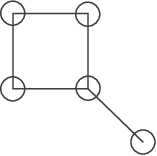
\includegraphics[scale=0.75]{pascal_2008_24.png}
        \end{center}        
\end{frame}


\refstepcounter{problem}
\begin{frame}[t, fragile]{Problem \thesection.\theproblem}
    \begin{block}{}[Mathcounts Handbook 2020-21, \#228]
     Five fair coins are flipped. Those that land heads up are flipped again. After the second round of flips, what is the probability that all five coins are now tails up? Express your answer as a common fraction. 
     
    \end{block}
\end{frame}

\refstepcounter{problem}
\begin{frame}[t, fragile]{Problem \thesection.\theproblem}
    \begin{block}{}[BmMT 2017]
    A gorgeous sequence is a sequence of 1’s and 0’s such that there are no consecutive 1’s. For
    instance, the set of all gorgeous sequences of length 3 is $ \{[1, 0, 0], [1, 0, 1], [0, 1, 0], [0, 0, 1], [0, 0, 0]\} . $
    Determine the number of gorgeous sequences of length 7.
    
    \end{block}
\end{frame}
% \newpage

\section{Challenge Practice Problems}
\refstepcounter{problem}
\begin{frame}[t, fragile]{Problem \thesection.\theproblem}
    \begin{block}{}[Mandelbrot National 2009]
    How many positive integers from 1 to 2009 have the property that, when tripled, they give a result having all even digits? 
    
    \end{block}
\end{frame}

\refstepcounter{problem}
\begin{frame}[t, fragile]{Problem \thesection.\theproblem}
    \begin{block}{}[Mathcounts]
     Two red, two yellow, and two green faces, all unit squares, are available for building a cube. How many distinct cubes can be built?
     
    \end{block}
\end{frame}

\refstepcounter{problem}
\begin{frame}[t, fragile]{Problem \thesection.\theproblem}
    \begin{block}{}[BmMT 2018 \#19]
Six people sit around a round table. Each person rolls a standard 6-sided die. If no two people sitting next to each other rolled the same number, we will say that the roll is valid. How many different rolls are valid?
% Answer: 15630
	
    \end{block}
\end{frame}

\refstepcounter{problem}
\begin{frame}[t, fragile]{Problem \thesection.\theproblem}
    \begin{block}{}[MATHCOUNTS 2013-14 Handbook, \#269]
Two standard six-sided dice, each with faces numbered with the positive integers 1 through 6, have the probability distribution shown for the sum of the top-facing values on the dice. Two non-standard but fair six-sided dice can be numbered differently with nonnegative integers on each face and still yield the same probability distribution. Though a number may be on both dice, a number may not appear more than once on either die. If $a$ is the sum of the six numbers on one of these non-standard dice, and $b$ is the sum of the six numbers on the other die, what is the value of the product $a \times b$?

    \end{block}
    \begin{center}
        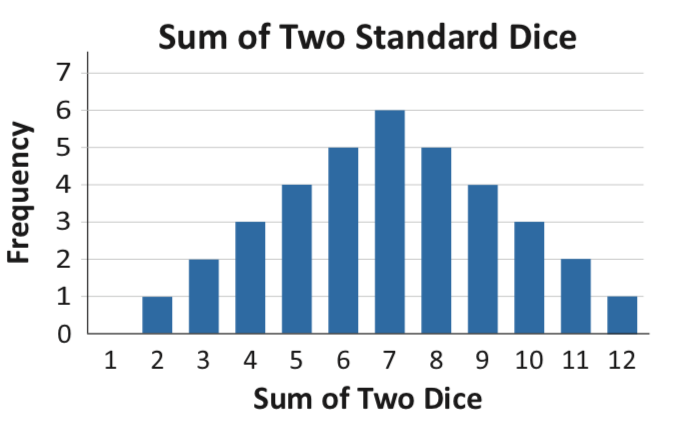
\includegraphics[scale=0.6]{images/hb13_169.png}
    \end{center}
    
\end{frame}

\refstepcounter{problem}
\begin{frame}[t, fragile]{Problem \thesection.\theproblem}
    \begin{block}{}[EMCC 2017]
Nicky likes dolls. He has 10 toy chairs in a row, and he wants to put some indistinguishable dolls on
some of these chairs. (A chair can hold only one doll.) He doesn’t want his dolls to get lonely, so he
wants each doll sitting on a chair to be adjacent to at least one other doll. How many ways are there
for him to put any number (possibly none) of dolls on the chairs? Two ways are considered distinct if
and only if there is a chair that has a doll in one way but does not have one in the other.
% Solution. The answer is 200 .


    \end{block}
\end{frame}

\end{document}
